\documentclass{article}
\usepackage[utf8]{inputenc}
\usepackage{graphicx}
\usepackage{here}

\title{Notes TC4}
\author{Adrien Pavao}
\date{September 2017}

\begin{document}

\maketitle

\tableofcontents

\section{Définitions et formules}

\subsection{Notions générales}

\begin{itemize}
\item \textbf{Variable aléatoire :} Une fonction définie depuis l'ensemble des résultats possibles d'une expérience aléatoire, dont on doit pouvoir déterminer la probabilité qu'elle prenne une valeur donnée ou un ensemble donné de valeurs. 

Cette variable peut être discrète ou continue.

Dans le cas d'une variable discrète, la fonction masse est la fonction qui donne la probabilité d'un résultat élémentaire d'une expérience.

Dans le cas d'une variable continue, la distribution de la masse de probabilité est caracterisée par la densité de probabilité f(x) : 

$ P(a < X \leq b)  = \displaystyle \int_{a}^{b} f(x) \, \mathrm{d}x  $

\item \textbf{Réalisations :} Les réalisations d'une variable aléatoire sont les résultats des valeurs choisies au hasard en fonction de la loi de probabilité de la variable. On les appelle également les variations aléatoires.

\item \textbf{Distribution (loi de probabilité) :} Le concept de loi de probabilité se formalise mathématiquement à l'aide de la théorie de la mesure : une loi de probabilité est une mesure, souvent vue comme la loi décrivant le comportement d'une variable aléatoire, discrète ou continue. Une mesure est une loi de probabilité si sa masse totale vaut 1. L'étude d'une variable aléatoire suivant une loi de probabilité discrète fait apparaître des calculs de sommes et de séries, alors que si sa loi est absolument continue, l'étude de la variable aléatoire fait apparaître des calculs d'intégrales.

\item \textbf{Inférence :} Trouver la valeur des v.a. à partir d'autres qui sont connues.

\item \textbf{Vraisemblance :} $P(D; \Theta)$ avec D les données d'estimation et $\Theta$ l'ensemble des paramètres.

\item \textbf{Estimation :} Retrouver les paramètres d'une distribution à partir de l'observation d'un ensemble de réalisations de celle-ci. Il s'agit du maximum de vraisemblance.

\item \textbf{Sampling :} Générer des données.

\end{itemize}

\subsection{Différentes probabilités liées}

\begin{itemize}

\item \textbf{Probabilité jointe :} Probabilité d'une configuration donnée. On note $P(X, Y)$. Il s'agit de la probabilité de la réalisation de l'évenement X \textbf{et} de l'évenement Y.

\item \textbf{Probabilité conditionnelle :} La probabilité de X sachant Y se note $P(X|Y)$. Pour faire simple, on fixe la variable connue.

$ P(X|Y) = \frac{P(X, Y)}{P(Y)} $
 
\item \textbf{Probabilité marginale :} On vire une variable en la sommant. A partir de $P(X = x, Y = y)$, on peut obtenir :

$ P(X = x) = \sum_{y} P(X = x, Y = y) $

\end{itemize}

La probabilité jointe inclus les deux autres. On peut retrouver la distribution jointe à partir de la distribution conditionnelle et
marginale.


\subsection{Moyenne, variance, covariance et corrélation}

Soit $x_1$, $x_2$, ..., $x_n$ un ensemble de valeurs générées par une distribution de probabilité inconnue. On peut caractériser cette distribution par : 

\begin{itemize}
\item La \textbf{moyenne}, qui caractérise le \textbf{centre} de la distribution.

$ \bar{x} = \frac{1}{n} \sum_{i=1}^{n} x_i $

\item La \textbf{variance}, qui mesure la \textbf{dispersion} de la distribution.

\begin{itemize}

\item $ \frac{1}{n} \sum_{i=1}^{n} (x_i - \bar{x})^{2} $

\item $ var(x) = \frac{1}{N} \sum_{n=1}^{N} (x_n - \bar{x})^2 $

\end{itemize}

\item L'\textbf{écart-type}, qui est la racine carrée de la variance.

$\sigma = \sqrt{var(x)}$

\item La symétrie ou l'asymétrie (skewness).

\begin{figure}[H]
   \caption{Schéma représentatif de la skewness}
    \begin{center} 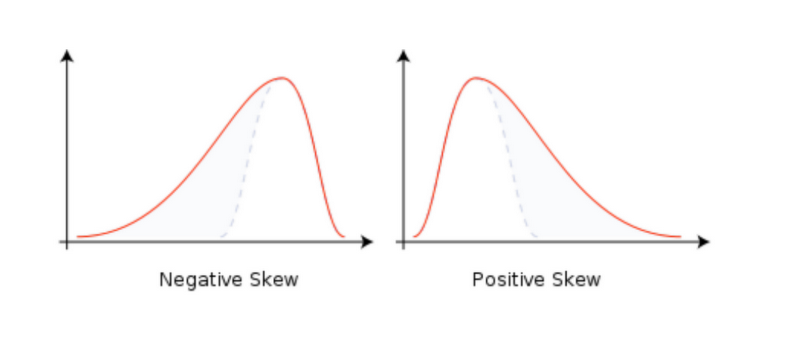
\includegraphics[scale=0.4]{skewness.png} \end{center}
\end{figure}


\item La covariance, le lien entre les variations de deux variables.

$ cov(x, y) = \frac{1}{N} \sum_{n=1}^{N} (x_n - \bar{x}) (y_n - \bar{y}) $

\item La corrélation, une covariance normalisée. Elle quantifie la qualité de l'approximation linéaire de x par y, et reciproquement.

$ cor(x, y) = \frac{cov(x, y)}{var(x) var(y)} = \frac{cov(x, y)}{cov(x, x) cov(y, y)} $


\end{itemize}


Pour les V.A. multidimensionnelles, on a la \textbf{matrice de covariance}.

\subsection{Indépendance statistique}

\begin{itemize}

\item \textbf{Variables indépendantes :} Deux variables sont indépendantes si et seulement si :

$ P(X = x, Y = y) = P(X = x) \times P(Y = y) $

\item \textbf{Variables conditionnellement indépendantes :} Deux variables sont conditionnellement indépendantes si et seulement si :

$ P(X = x, Y = y | Z = z) = P(X = x | Z = z) \times P(Y = y | Z = z) $

\item \textbf{Indépendantes et identiquement distribuées (i.i.d) :} Ce dit de deux variables indépendantes suivant la même loi de probabilité. Il sera souvent nécessaire de poser cette hypothèse. On en déduit : $P(X_{1, N} ) = \prod_{1}^{N} P(X_i)$

\end{itemize}

\subsection{Théorème de Bayes}

\begin{itemize}

\item $ P(Y = y_j | X = x_i) = \frac{P(X = x_i | Y = y_j) P(Y = y_j)}{\sum_{y_j \in A_y} P(X = x_i | Y = y_j) P(Y = y_j)}  $

\item $ P(Y = y_j | X = x_j) = \frac{P(X = x_i | Y = y_j) P(Y = y_j)}{P(X = x_i)} $

\end{itemize}

\subsection{Lois de probabilités courantes}

\begin{tabular}{|l|l|c|l|}
  \hline
  Loi & Type de la V.A. & Formule & Paramètres \\
  \hline
  Bernouilli & Binaire & $p^x(1-p)^{1-x}$ & p \\
  Binomiale & Discrète & $C^{k}_{n} \times p^k \times (1-p)^{n-k}$ & n, p \\
  Poisson &Discrète & $\frac{\lambda^k}{k!} \times e^{- \lambda} $ & $\lambda$ \\
  Normale dimension 1 & Continue & $\frac{1}{\sigma \sqrt{2 \pi}} \times e^{\frac{-1}{2}(\frac{x - \mu}{\sigma})^2} $ & $\mu$, $\sigma$ \\
  Normale dimension d & Continue& $\frac{1}{(2 \pi)^{\frac{d}{2}} ||\Sigma||^{\frac{1}{2}}} \times e^{- \frac{1}{2} (x - \mu)^t \Sigma^{-1} (x - \mu)}$ & $\mu$, $\Sigma$ \\ 
  \hline
\end{tabular}


\section{Classification bayésienne}

Note : A completer.

Soit les points suivantes:

\begin{itemize}
\item Variable aléatoire X, une observation à classer.
\item Variable aléatoire Y, désignant la classe à affecter à X.
\item Décision $\alpha_i$, affectation de x à la classe $y = i$.
\item Fonction de perte $\lambda(\alpha_i | j)$, décision $\alpha_i$ alors que la classe correcte était j.
\end{itemize}

Sur l'observation x, l'espérance du risque de décider $\alpha_i$ est : 

$ R(\alpha_i | x) = \sum_{j = 1}^{k} \lambda(\alpha_i | j) P(Y = j | x) $

\end{document}

